\documentclass[tikz,border=3pt]{standalone}
\usepackage{mathptmx}
\usetikzlibrary{arrows.meta,decorations.pathmorphing}
\newcommand{\bladeLabel}{Palas flexibles}
\newcommand{\towerLabel}{Torre flexible}
\newcommand{\nacelleLabel}{Góndola}
\newcommand{\hubLabel}{Cubo}
\newcommand{\trainLabel}{Tren elástico}
\newcommand{\baseLabel}{Base / cimentación}
\begin{document}
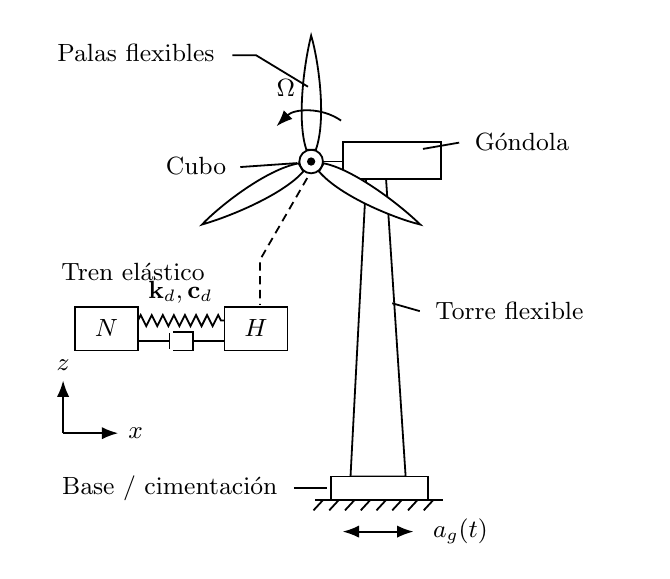
\begin{tikzpicture}[x=1cm,y=1cm,>=Latex,font=\small,line width=.65pt]
\path[use as bounding box](-.3,-.45) rectangle (7.5,6.2);
% Tower and nacelle, rear of the rotor.
\draw[fill=white](3.8,.5)--(4.0,4.3)--(4.25,4.3)--(4.5,.5)--cycle;
\draw[fill=white](3.7,4.28) rectangle (4.95,4.75);
\draw (3.4,4.5)--(3.7,4.5);
\draw[fill=white](3.3,4.5) circle(.15);
% Three tapered blades.
\foreach \a in {90,210,330}{
  \begin{scope}[shift={(3.3,4.5)},rotate=\a]
    \draw[fill=white](.15,-.06) .. controls (.55,-.20) and (1.3,-.09) .. (1.6,0)
       .. controls (1.2,.10) and (.5,.18) .. (.15,.06)--cycle;
  \end{scope}}
\fill (3.3,4.5) circle(1.5pt);
\draw[->](3.68,5.02) arc(55:135:.64);
\node at (2.98,5.43){$\Omega$};
\node[anchor=west] at (-.05,5.88){\bladeLabel};
\draw (2.3,5.85)--(2.6,5.85)--(3.26,5.45);
\node[anchor=west] at (5.25,4.75){\nacelleLabel};
\draw(4.72,4.66)--(5.18,4.74);
\node[anchor=east] at (2.35,4.44){\hubLabel};
\draw(2.4,4.43)--(3.12,4.48);
\node[anchor=west] at (4.75,2.6){\towerLabel};
\draw(4.33,2.7)--(4.68,2.6);
\draw[fill=white](3.55,.20) rectangle(4.78,.50);
\draw(3.35,.20)--(4.98,.20);
\foreach \xx in {3.45,3.65,3.85,4.05,4.25,4.45,4.65,4.85}{\draw(\xx,.20)--++(-.12,-.13);}
\node[anchor=east] at (3.0,.35){\baseLabel};
\draw(3.08,.35)--(3.50,.35);
\draw[<->](3.7,-.2)--(4.6,-.2);
\node[anchor=west] at (4.72,-.2){$a_g(t)$};
% Expanded connection diagram.
\node[anchor=west] at (.0,3.1){\trainLabel};
\draw[fill=white](.3,2.1) rectangle(1.1,2.65);
\draw[fill=white](2.2,2.1) rectangle(3.0,2.65);
\node at (.7,2.38){$N$};\node at (2.6,2.38){$H$};
\draw[decorate,decoration={zigzag,segment length=4pt,amplitude=2pt}](1.1,2.48)--(2.2,2.48);
\draw (1.1,2.22)--(1.50,2.22);\draw(1.5,2.12)--(1.5,2.32);
\draw(1.55,2.10)--(1.8,2.10)--(1.8,2.34)--(1.55,2.34);
\draw(1.8,2.22)--(2.2,2.22);
\node at (1.64,2.84){$\mathbf k_d,\mathbf c_d$};
\draw[densely dashed](3.25,4.29)--(2.65,3.25)--(2.65,2.68);
\draw[->](.15,1.05)--(.85,1.05)node[right]{$x$};
\draw[->](.15,1.05)--(.15,1.72)node[above]{$z$};
\end{tikzpicture}

\end{document}
